\section{\osrank{}}
\label{s:osrank}

\def\Graph{\mathsf{Graph}}
\def\proj{\mathsf{proj}}
\def\user{\mathsf{user}}
\def\dep{\mathsf{dep}}
\def\own{\mathsf{own}}
\def\contrib{\mathsf{contrib}}
\def\cocontrib{\mathsf{contrib}^\circ}

One of the fundamental mechanisms of \oscoin{} is to distribute a
portion of newly minted tokens to high-value projects on the
network. For this we need concensus on which projects are ``high
value''.  To choose which projects receive compensation, and in which
proportions, the network uses \osrank{}, which is a modification of
the well-know \pagerank{} algorithm \cite{pagerank} applied to the
graph of relationships between projects on the network, for example
\emph{dependencies}. The output of the algorithm is a score associated
to each project. Newly minted tokens are then distributed to projects
proportionally to their score.

\subsection{Rationale}

There are many systems in which value is produced. However, while it
may be clear that value is being produced by the system as a whole, it
is often unclear what value particular subsystems are
contributing. Furthermore, subsystems have inherently differing
capacities to transform value into revenue: subsystems at the
boundaries with other domains are at an advantage, even though they
may (transitively) derive much of their value from other
subsystems. This disbalance in value flows in and out of subsystems is
detrimental to the system as a whole.

Thankfully, human activity does not happen in a void\footnote{Space
  exploration will be addressed in a subsequent paper.}: be it
knowledge work, content/media creation, financial activity, etc.,
entities interact with one another in meaningful ways that are highly
influenced by the relative value each entity has with respect to the
system as a whole. Crucially, during this activity, a trail of
\emph{artefacts} (hypermedia links, contracts, transactions,
dependencies, pull-requests etc.) is produced; concrete manifestations
of the relationships between the various entities.

The basic insight of \pagerank{} and similar metrics, is that by
stochastic simulation of meaningful activity traces of system agents,
producing trails of artefacts consistent with observations, one can
learn about the value flows between subsystems, and hence approximate
a projection of the underlying value distribution. In the case of
\pagerank{} one simulates a human searching for high-relevance data over
the internet, following a chain of links. A sophisticated algorithm
would use as many heuristics as possible for choosing the next link to
follow (as a real human would), e.g.\ evaluating the relevance of the
link-text. If computational resources are scarce, the crudest
algorithm simply picks the next link at random, and this is what
produces the classic \pagerank{} formula which has seen so much
success at ranking web pages.

In the domain of open source software development, the main artefacts
produced are:
\begin{itemize}
  \item Build-dependencies between projects,
  \item Contributions of PRs from programmers to projects.
  \item Reviews and merges of PRs by maintainers into projects.
  \item ? % TODO:
\end{itemize}

We summarise this by the following weighted directed graph $G$, the
weights corresponding to the relative importance of the activity,
tweaked by our own judgement and informed by simulations we have run.

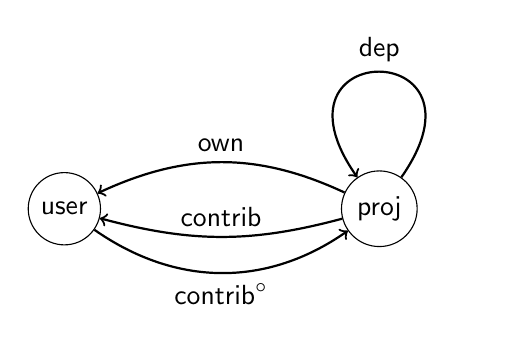
\begin{tikzpicture}[vertex/.style={draw,circle}, arr/.style={draw,thick,->}]
  \node[vertex] (p) at (2,0) {$\proj$};
  \node[vertex] (u) at (-2,0) {$\user$};

  \draw[arr,looseness=10] (p) to[out=55,in=125] node[above] {$\dep$} (p);
  \draw[arr] (p) to[out=155,in=25] node[above] {$\own$} (u);
  \draw[arr] (p) to[out=195,in=-15] node[above] {$\contrib$} (u);
  \draw[arr] (u) to[out=-35,in=215] node[below] {$\cocontrib$} (p);
\end{tikzpicture}

We are using the following weights:
\begin{center}
  \begin{tabular}{lr}
  edge & weight \\
  \hline
  $\dep$ & $1.0$ \\
  $\own$ & $0.8$ \\
  $\contrib$ & $0.4$ \\
  $\cocontrib$ & $0.2$
  \end{tabular}
\end{center}

Note that contributions are counted as a bidirectional flow: a
contribution of a user to a project, $\contrib$, indicates that a user
has added value to a project. The flow in the opposite direction,
$\cocontrib$, is taken as an indication that the project is valuable
to the user: users are likely to contribute to projects they find
valuable.

% TODO: include similations data.

The \oscoin{} network proposes to record these artefacts as
transactions in a blockchain, so that one may unambiguously rebuild
(and reach consensus on) a finite directed graph $X$ over $G$ (i.e.,
in the slice category $\Graph/G$). We'll refer to $X$ as the
\emph{network graph}.

This in turn allows global value scores to be assigned to entities
according to a specific stochastic process simulating \emph{random
  walks}, that is, activity traces in $X$ with sampling probabilities
taken by projecting to $G$. For example: a contributor decides to work
on a high value project (probably at the border), contributes a PR, in
so doing adds a dependency to another project, which imports a bug
from upstream. The contributor therefore switches to fixing said bug
in the dependency, etc. Much like a simulation of a human searching
for information by clicking through links, this simulated contributor
activity informs us on the value flows between subsystems in OSS
development.

This score, which we call \osrank{}, is used to weight the
distribution of newly minted tokens to high value entities, thus
compensating entities which bring value to the ecosystem.

More specifically we use the following Monte Carlo-based algorithm:
for each project on the network, $R$ random walks are performed which
start at that node and proceed by sampling outgoing edges, according
to the weights declared in $G$. At each step the walk might terminate
with probability $1 - \epsilon$, (here $\epsilon$ is the \emph{damping
  factor}, $0 < \epsilon < 1$). This produces a set $W$ of walks. The
\osrank{} for a project $x$ is then:
\[
  s(x) = \frac{W_x \epsilon}{n R}
\]
where $W_x$ is the number of visits of $x$, over all walks, that is:
\[
W_x = \sum_{w \in W} v(w,x)
\]
where $v(w,x)$ is the number of times path $w$ visits the vertex $x$.

\subsection{Potential problems}

The main problem to avoid is compensating fake ecosystems, that is,
project structures and relationships which have been setup in the
network graph for the sole purpose of gaming the \osrank{} algorithm.

For this we propose running \osrank{} in two distinct phases:
\begin{itemize}
\item In the first phase, a seed set $S$ is used as the for the
  beginning of all walks. Specifically, a random walk always starts at
  a vertex in $S$. Otherwise the process remains the same. The scores
  obtained are biased towards interactions with the seed set, but they
  are not used directly by the compensation mechanism. Instead a
  threashold $t$ is used to determine the legitimacy of entities: any
  entity falling below this threshold is not considered for the next
  phase. One obtains a subgraph of the network graph $X_t$.
\item In the seconds phase, the algorithm is ran on the subgraph $X_t$
  as usual, with no seed set. The output of the second phase is the
  \osrank{}.
\end{itemize}

% TODO: remove the term governance.
We propose that the seed set be maintained by an on-chain governance
system, aiming to choose high-value user-facing projects,
e.g. Firefox, Debian, VLC, etc. Care must be taken to ensure the seed
set is large enough to touch most legitimate projects on the network.

\subsection{Implementation}

There are several options for making sure the computation of \osrank{}
will not be prohibitively expensive for operators to run.

\begin{itemize}
\item \emph{Incremental Monte Carlo.} An incremental algorithm is used
  so that \osrank{} values may be updated as network graph
  evolves. Instead of computing \osrank{} from scratch, we rely on the
  fact that only a small percentage of the nodes and edges of the
  network graph are added or removed from one calculation to the next
  (confirmed empirically on the datasets of major code-hosting
  platforms). Therefore most of the random walks that were performed
  in the previous calculation remain valid in the updated graph. For
  example if only a single dependency $x \to y$ has been added, then a
  walk is invalid only if passes through $x$, for it may have chosen
  to follow this new dependency.

  In practice the operators of the network cache the set of random
  walks from the previous calculation, and update this set by removing
  invalid walks and replacing them with new ones. Details on such an
  incremental algorithm used in the case of \pagerank{} can be found
  in \cite{incr_pagerank}.

  Since all the computations must be deterministic, the walks are not
  truly random. Rather, they must use a built-in pseudo-random number
  generator to generate the random walks. The seed for generating
  random walks is fixed in the genesis block.

  % TODO: Add details on RNG

\item \emph{Long epoch.} In this scenario payouts according to
  \osrank{} are only made infrequently, say with a duration of $d$
  between \emph{payout} blocks (e.g.\ once every month). In this case
  abusers might modify network structures of several projects in
  anticipation of the payout block. To mitigate this, some edges are
  weighted by the amount of time it has existed in the last epoch. For
  example, if a dependency is added a day before the payout block,
  then it only has a wight proportional to $1/d$.
\end{itemize}

\subsection{Required transactions}

In order for \osrank{} to be computable, the operators need access to the network graph, and so the following transactions must be supported at the very least:
\begin{itemize}
\item Transactions for adding and removing projects.
\item Transactions for adding and removing users.
\item Transactions for adding and removing dependencies.
\item Transactions for stating a contribution of a user to a project.
\end{itemize}
For more details, see the ledger section. % TODO: add reference to
                                          % ledger section.
